% =====================================================================
% Supporting Information for the IJGGC CO2 depressurisation manuscript.
% Standalone document: the full model-versus-measurement comparison for
% all fifteen experiments (six CARDICE, nine SINTEF). Figures/tables are
% numbered S1, S2, ... No em-dashes anywhere (house rule).
% =====================================================================
\documentclass[preprint,authoryear,12pt]{elsarticle}

\usepackage[T1]{fontenc}
\usepackage{textcomp}
\usepackage{graphicx}
\usepackage{float}
\usepackage{amsmath}
\usepackage{amssymb}
\usepackage{hyperref}

% Supporting-information numbering (S1, S2, ...)
\renewcommand{\thefigure}{S\arabic{figure}}
\renewcommand{\thetable}{S\arabic{table}}
\renewcommand{\thesection}{S\arabic{section}}

\journal{International Journal of Greenhouse Gas Control}

\begin{document}

\begin{frontmatter}
\title{Supporting Information for: Modelling the depressurisation of CO$_2$ storage vessel at
conditions relevant for intermediate storage and transport}
\author[ors]{Anders Andreasen}
\address[ors]{ORS Consulting Aps, Borgergade 66 st th., DK-6700 Esbjerg, Denmark}
\end{frontmatter}

This Supporting Information collects the full set of model-versus-measurement comparisons for
all fifteen experiments used in the main paper: six CARDICE tests (numbers 5 to 10) and nine
SINTEF dense-phase tests. Each figure shows, for a single test, four panels: the vessel
pressure, the inventory with the modelled gas/liquid/solid breakdown, the internal fluid
temperature (the measured upper and lower bands together with the modelled gas and
liquid/solid temperatures), and the inside-wall temperature (the measured bands together with
the modelled gas-contact and wetted-wall nodes). In every panel the model is shown dashed and
the measured data solid. The test conditions and the aggregate results are given in the main
paper; the representative cases discussed there are tests 7 and 8 (CARDICE) and Exp72 and Exp53
(SINTEF).

% =====================================================================
\section{CARDICE (Ineris 2\,m$^3$ sphere)}

\begin{figure}[htbp]
\centering
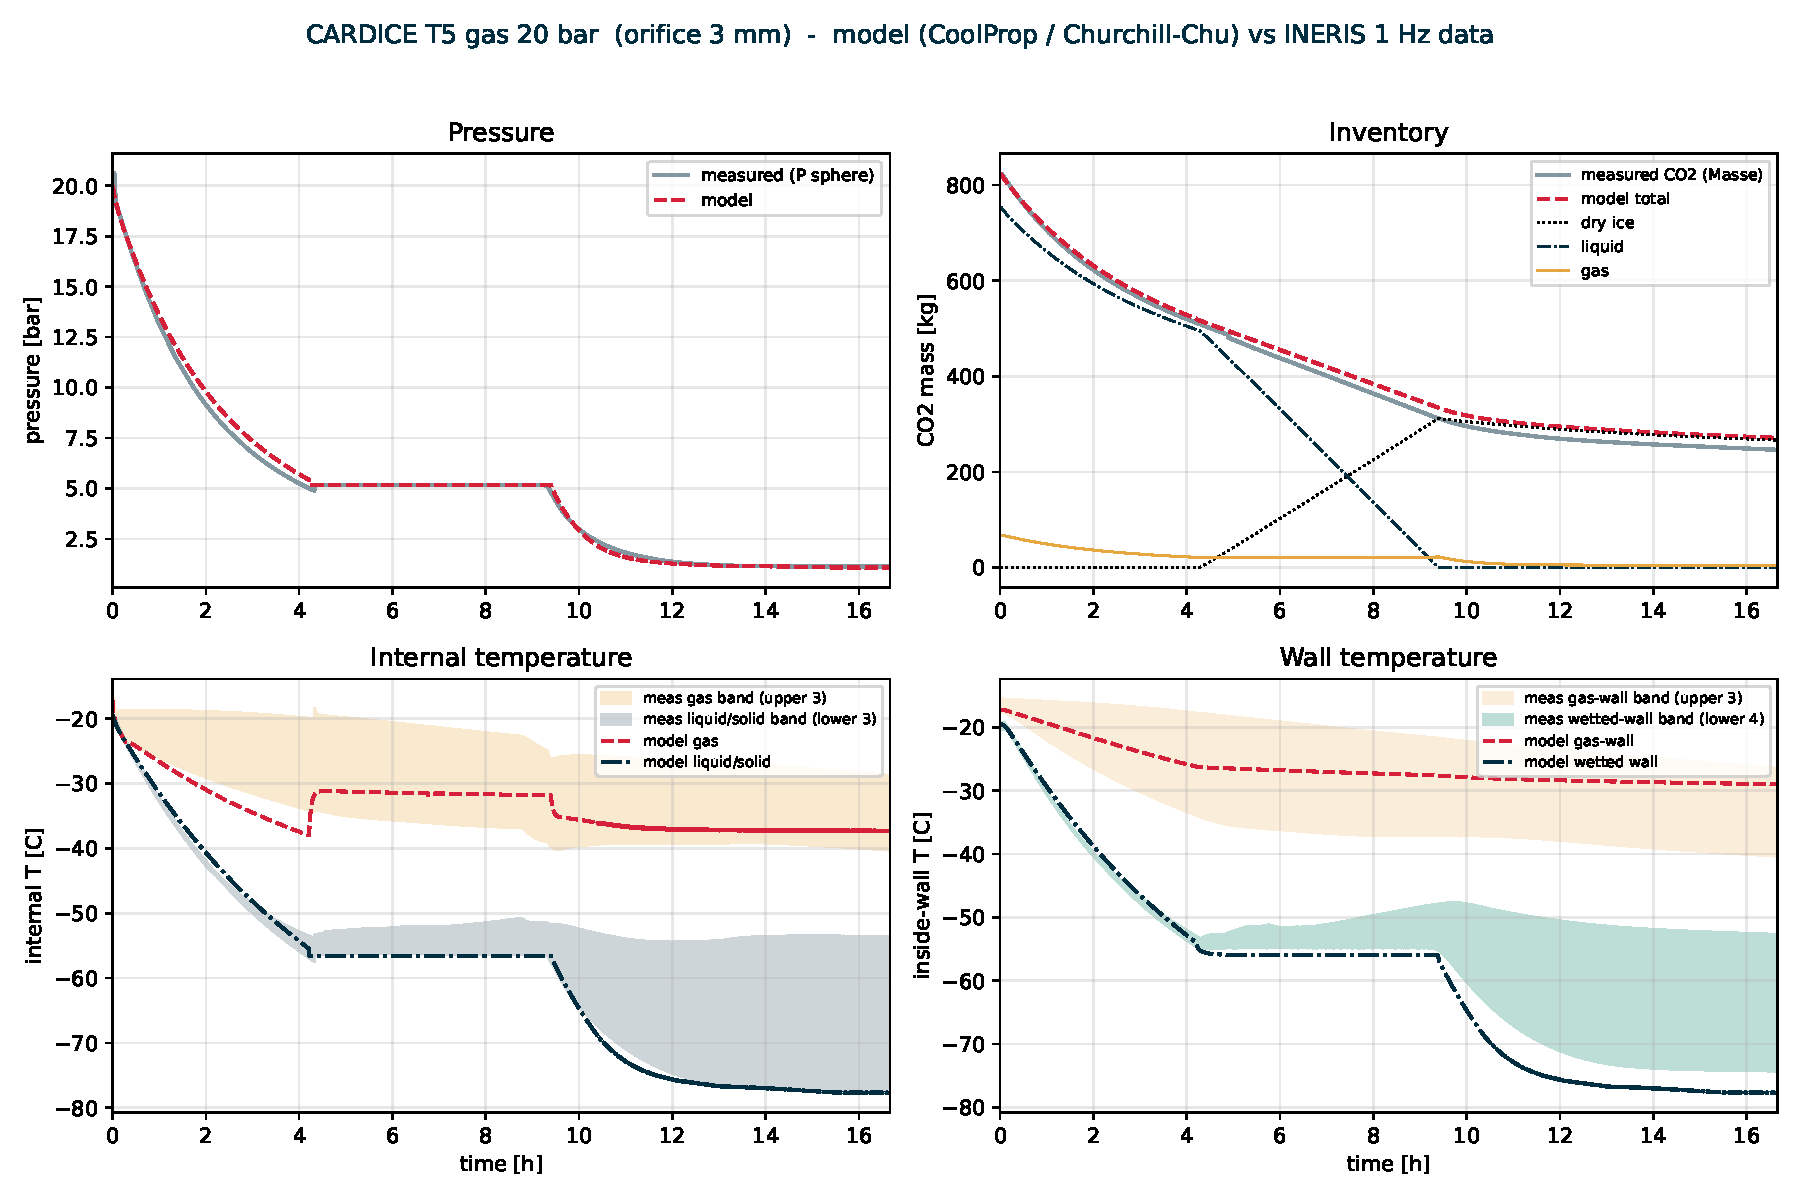
\includegraphics[width=\textwidth]{figures/cardice_t5}
\caption{CARDICE test~5: gas release, 20\,bar, $-20\,^\circ$C, 3\,mm orifice.}
\label{fig:si-t5}
\end{figure}

\begin{figure}[htbp]
\centering
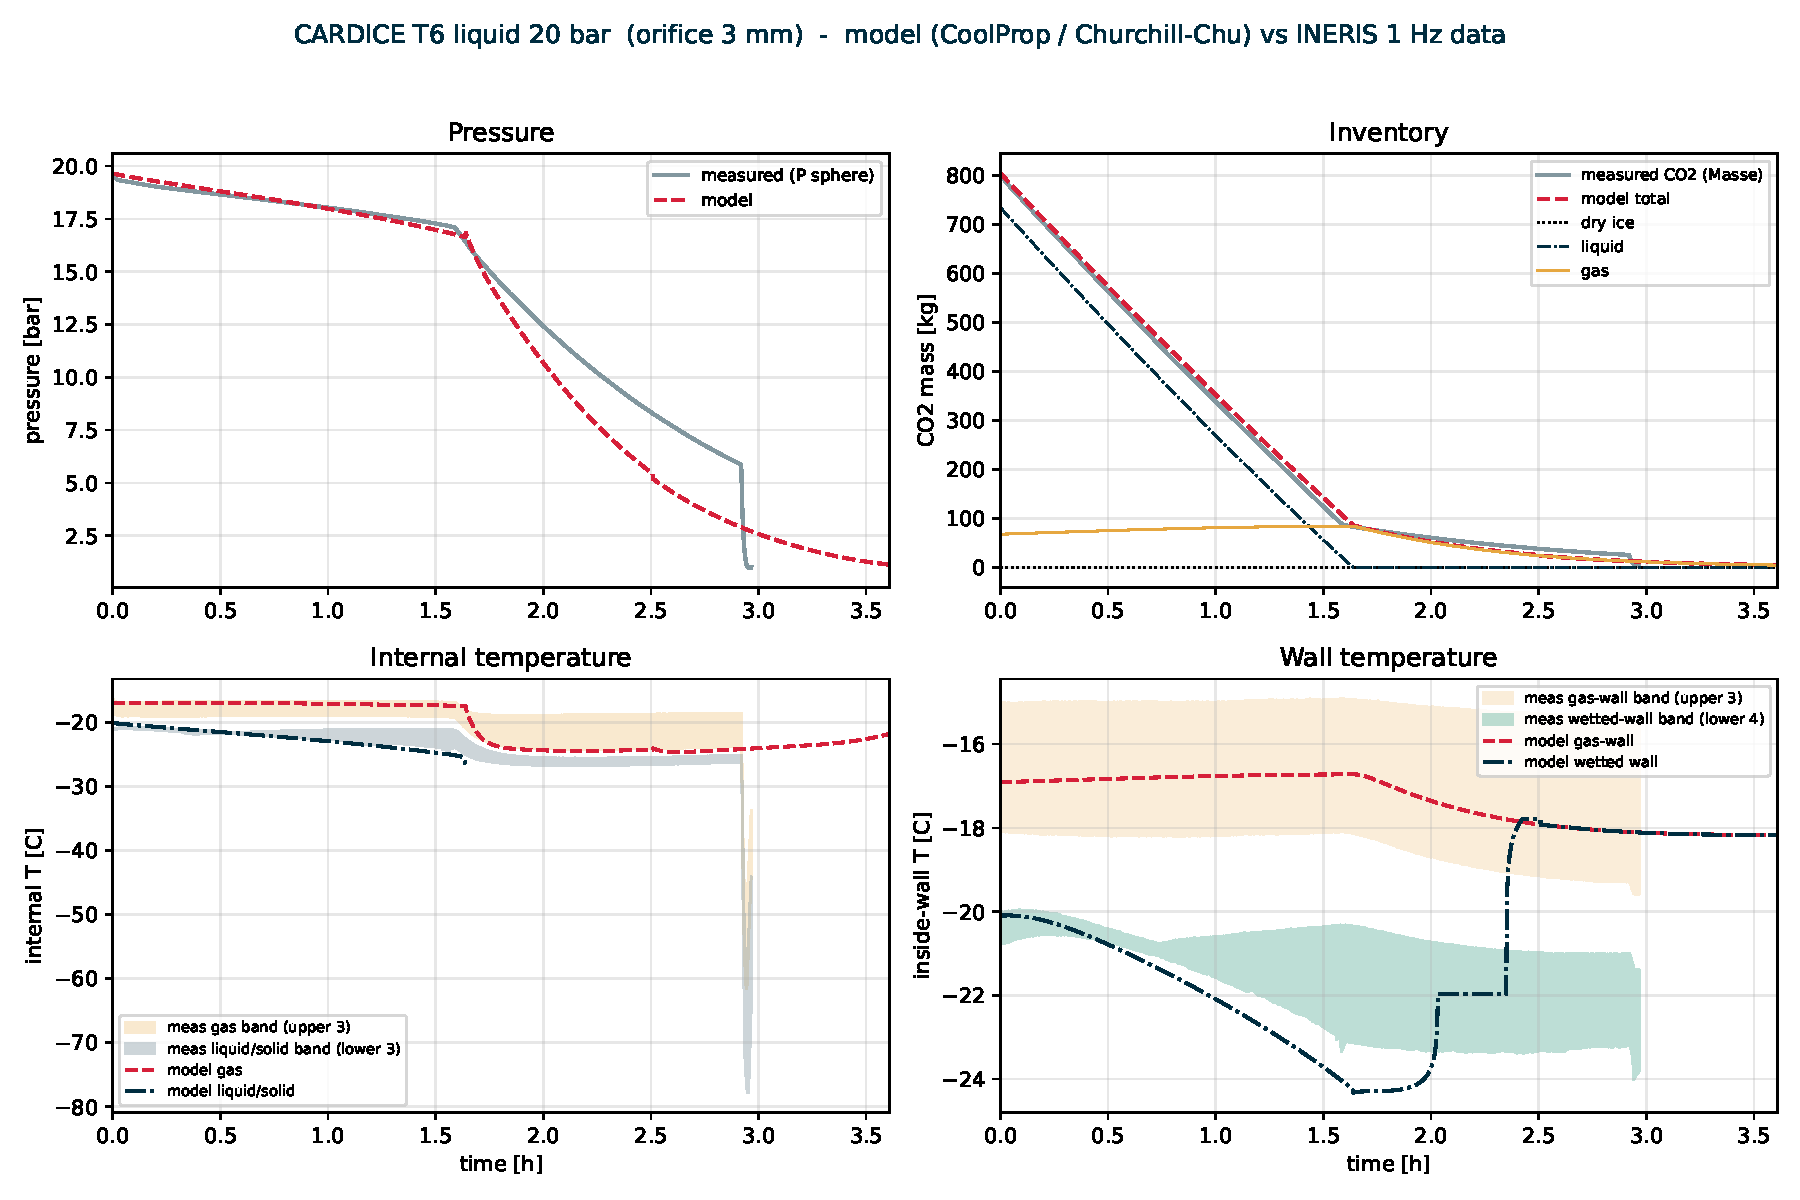
\includegraphics[width=\textwidth]{figures/cardice_t6}
\caption{CARDICE test~6: liquid release, 20\,bar, $-20\,^\circ$C, 3\,mm orifice.}
\label{fig:si-t6}
\end{figure}

\begin{figure}[htbp]
\centering
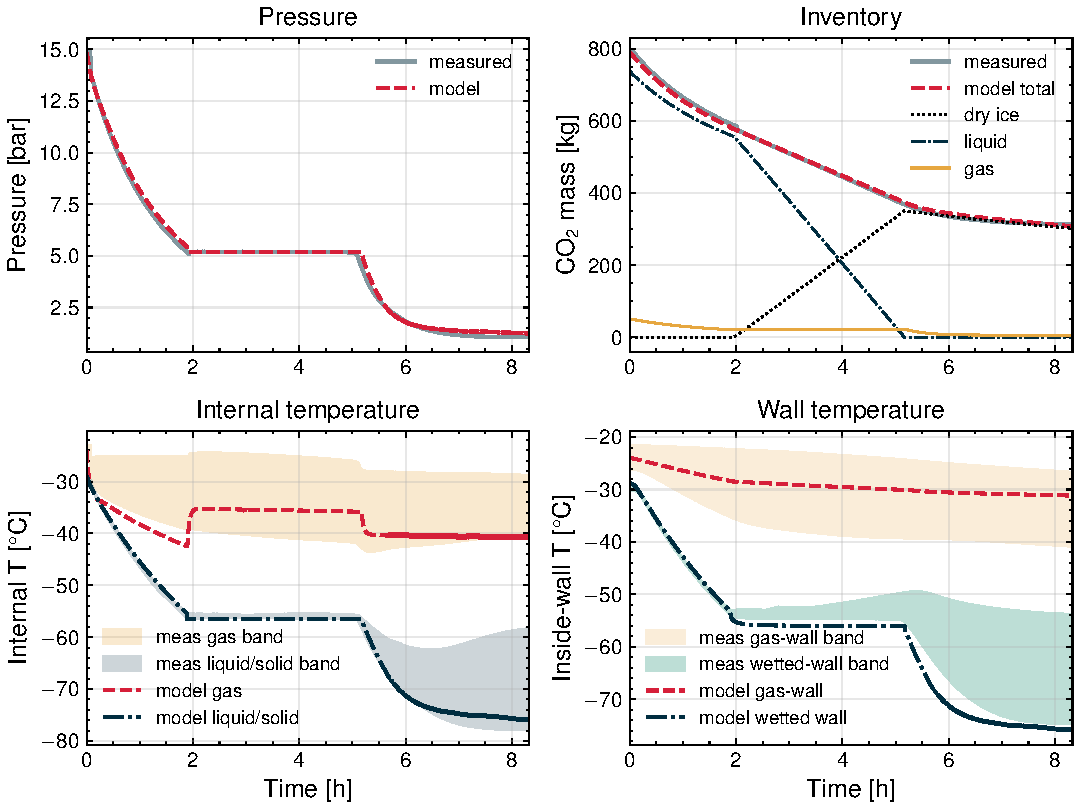
\includegraphics[width=\textwidth]{figures/cardice_t7}
\caption{CARDICE test~7: gas release, 15\,bar, $-29\,^\circ$C, 4\,mm orifice.}
\label{fig:si-t7}
\end{figure}

\begin{figure}[htbp]
\centering
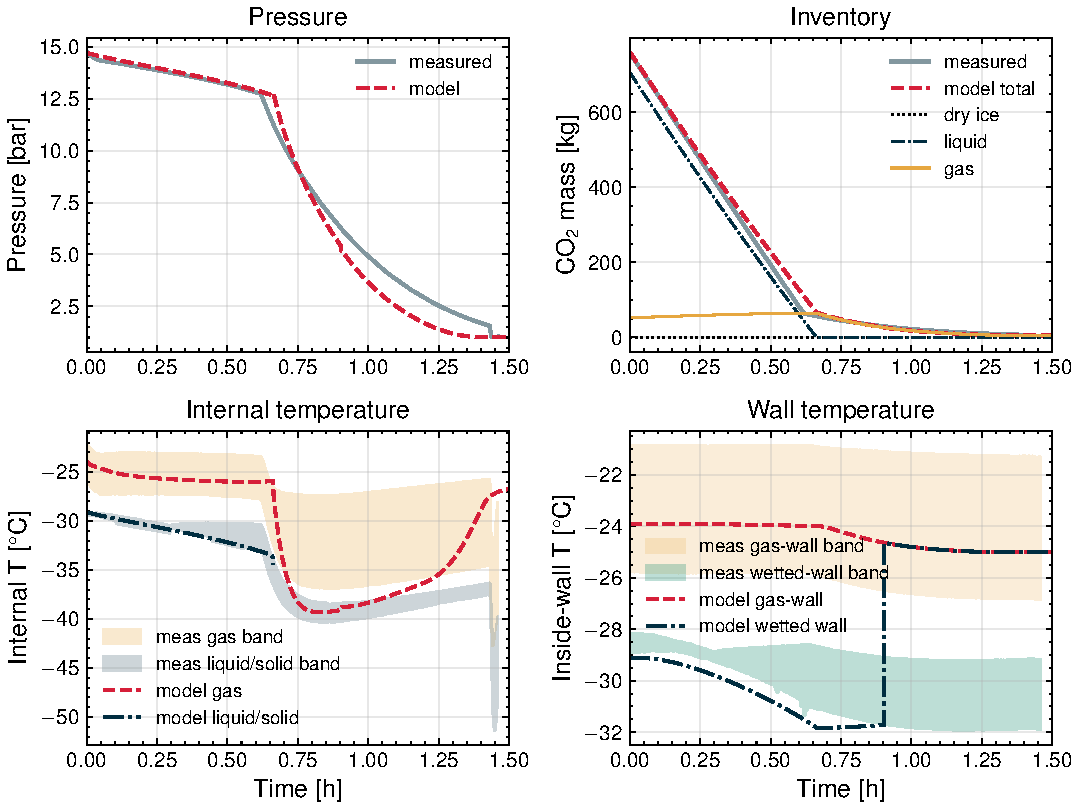
\includegraphics[width=\textwidth]{figures/cardice_t8}
\caption{CARDICE test~8: liquid release, 15\,bar, $-29\,^\circ$C, 5\,mm effective orifice.}
\label{fig:si-t8}
\end{figure}

\begin{figure}[htbp]
\centering
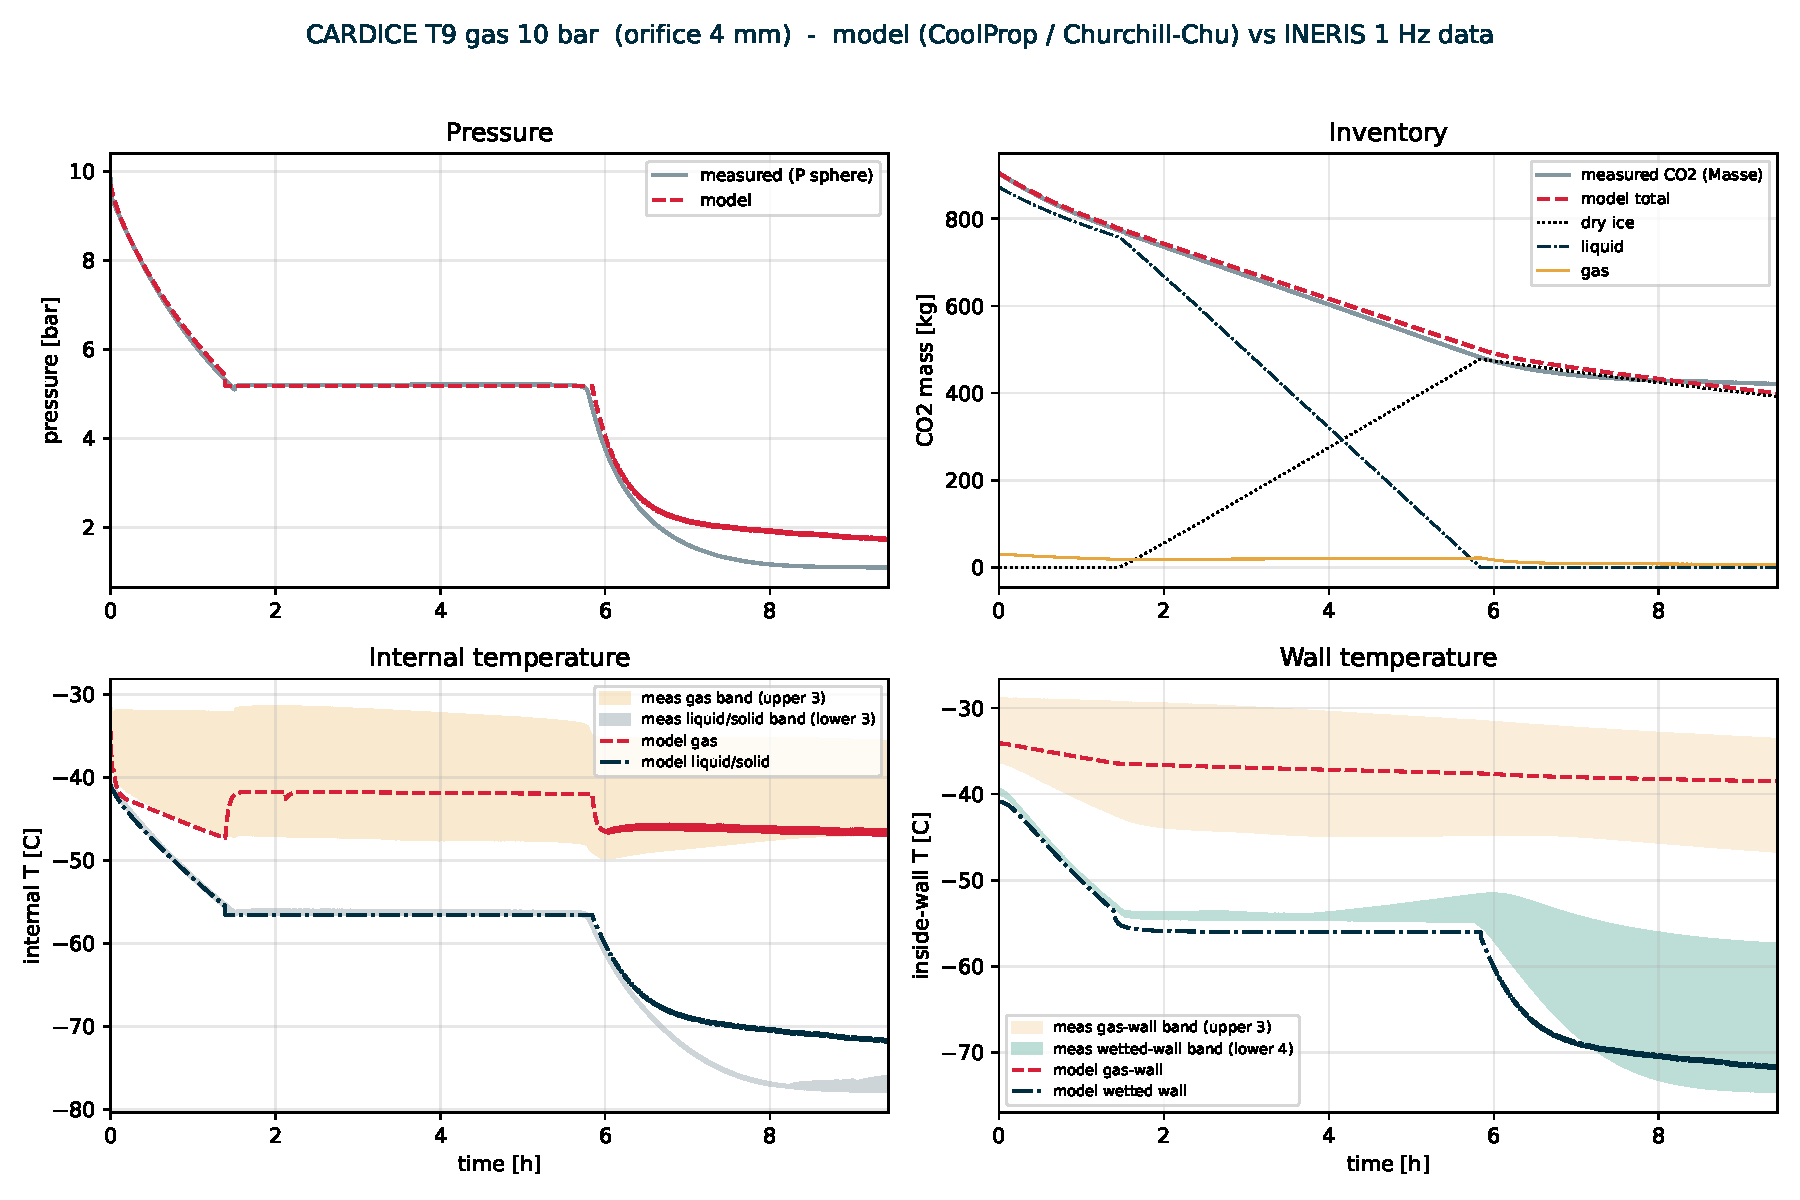
\includegraphics[width=\textwidth]{figures/cardice_t9}
\caption{CARDICE test~9: gas release, 10\,bar, $-40\,^\circ$C, 4\,mm orifice.}
\label{fig:si-t9}
\end{figure}

\begin{figure}[htbp]
\centering
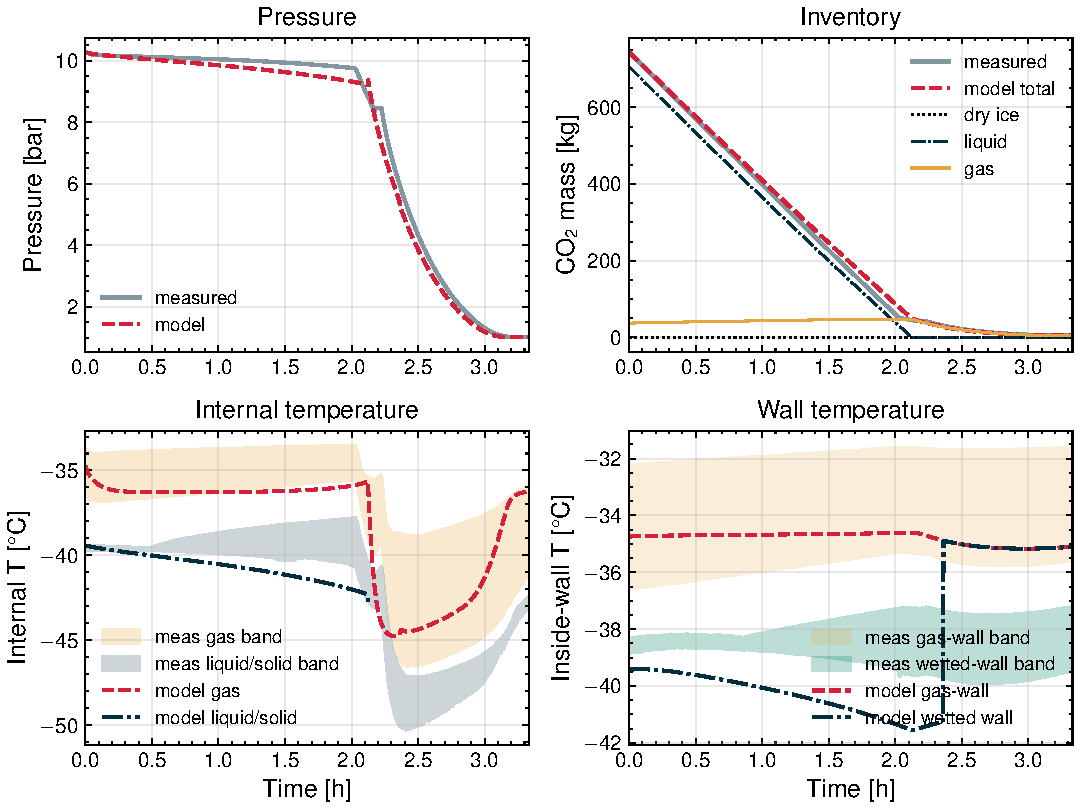
\includegraphics[width=\textwidth]{figures/cardice_t10}
\caption{CARDICE test~10: liquid release, 10\,bar, $-40\,^\circ$C, 4\,mm orifice.}
\label{fig:si-t10}
\end{figure}

% =====================================================================
\section{SINTEF dense-phase experiments}

\subsection*{No-riser (gas) releases}

\begin{figure}[htbp]
\centering
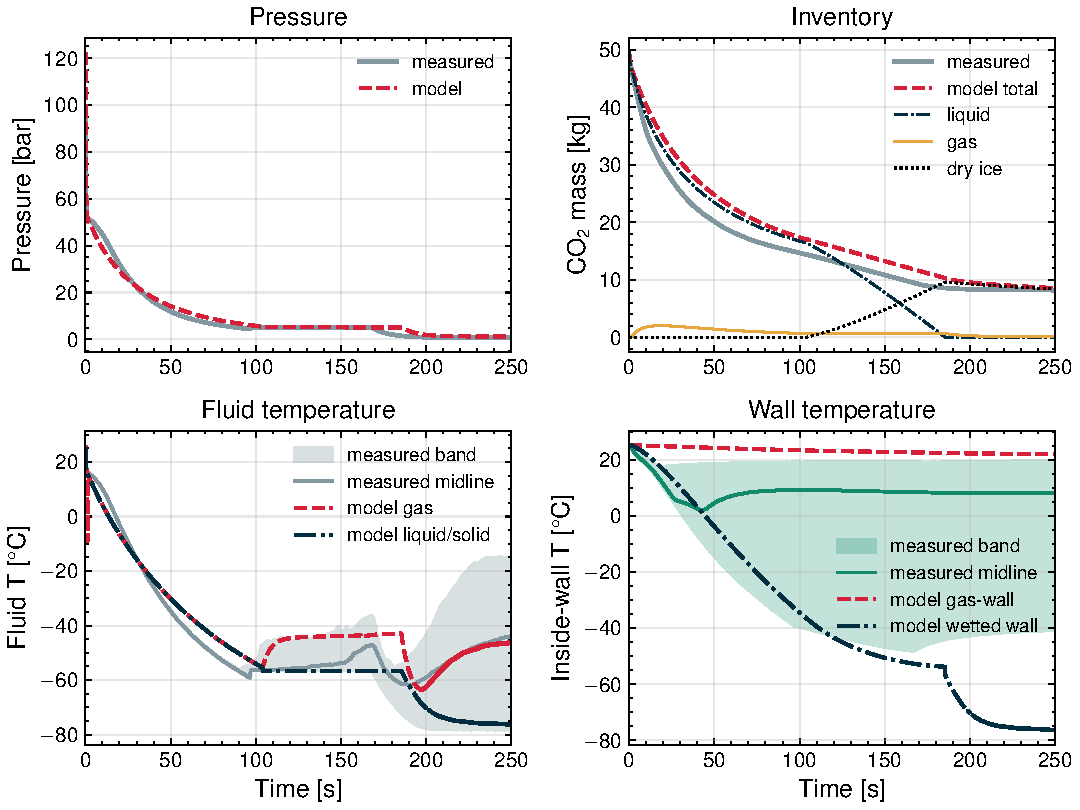
\includegraphics[width=\textwidth]{figures/munke_exp71}
\caption{SINTEF Exp71: no-riser (gas), 122.6\,bar, 25.2\,$^\circ$C, 8.0\,mm nozzle.}
\label{fig:si-exp71}
\end{figure}

\begin{figure}[htbp]
\centering
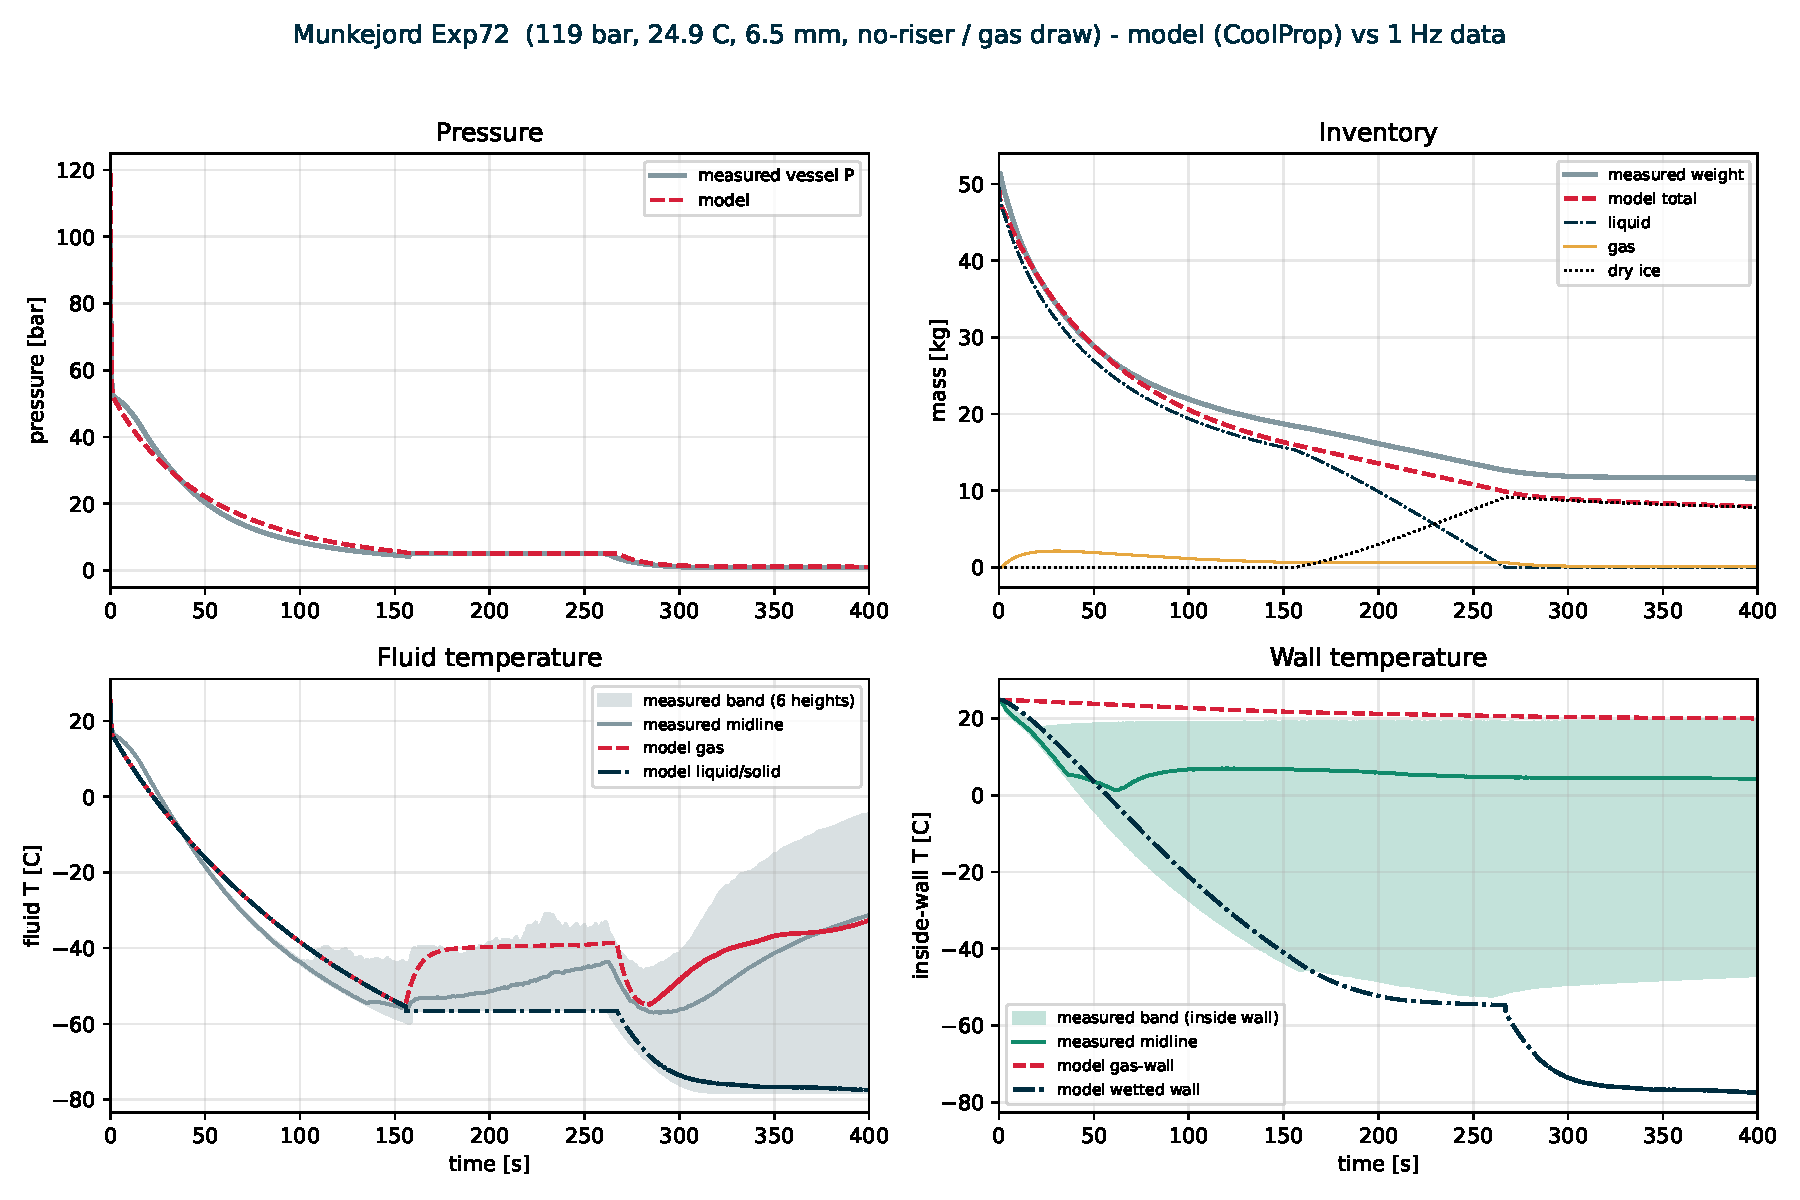
\includegraphics[width=\textwidth]{figures/munke_exp72}
\caption{SINTEF Exp72: no-riser (gas), 119.0\,bar, 24.9\,$^\circ$C, 6.5\,mm nozzle.}
\label{fig:si-exp72}
\end{figure}

\begin{figure}[htbp]
\centering
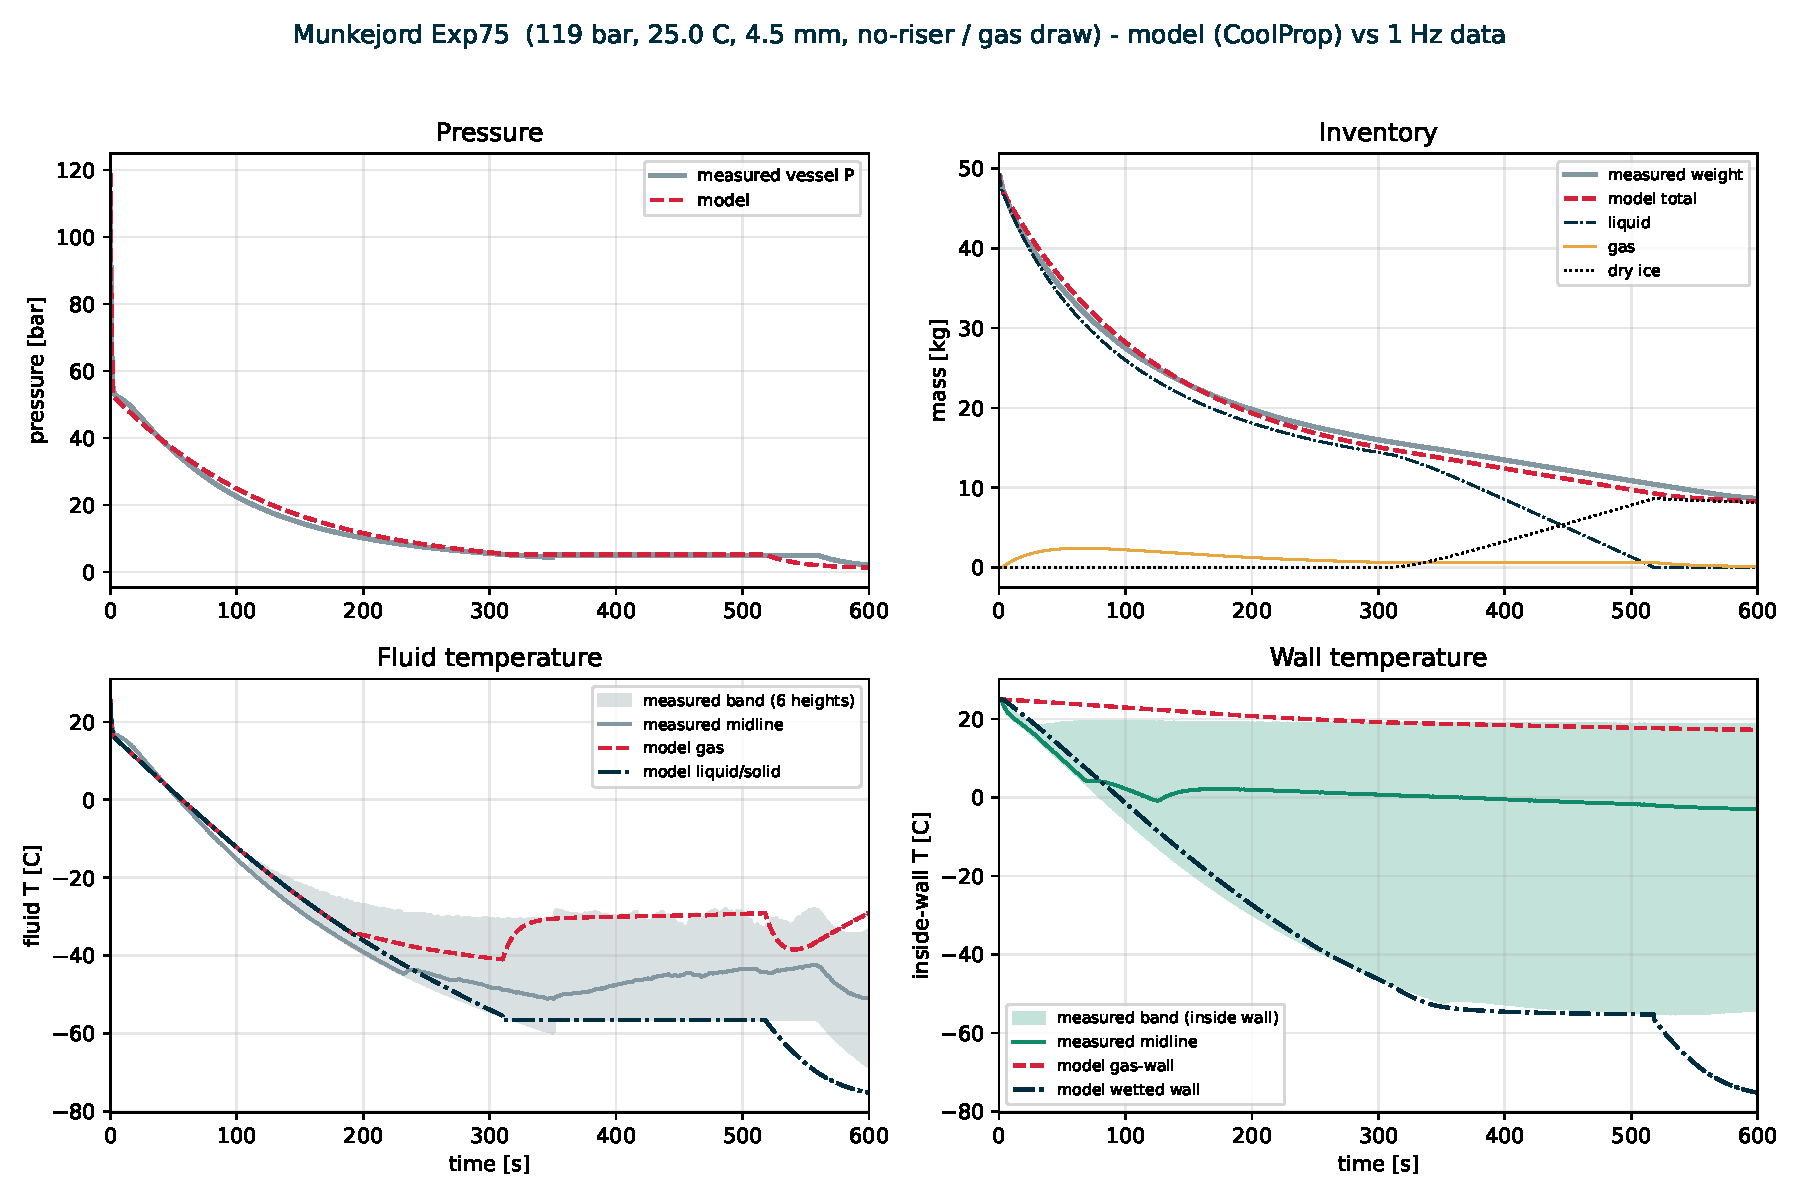
\includegraphics[width=\textwidth]{figures/munke_exp75}
\caption{SINTEF Exp75: no-riser (gas), 119.0\,bar, 25.0\,$^\circ$C, 4.5\,mm nozzle.}
\label{fig:si-exp75}
\end{figure}

\subsection*{Riser (liquid) releases}

\begin{figure}[htbp]
\centering
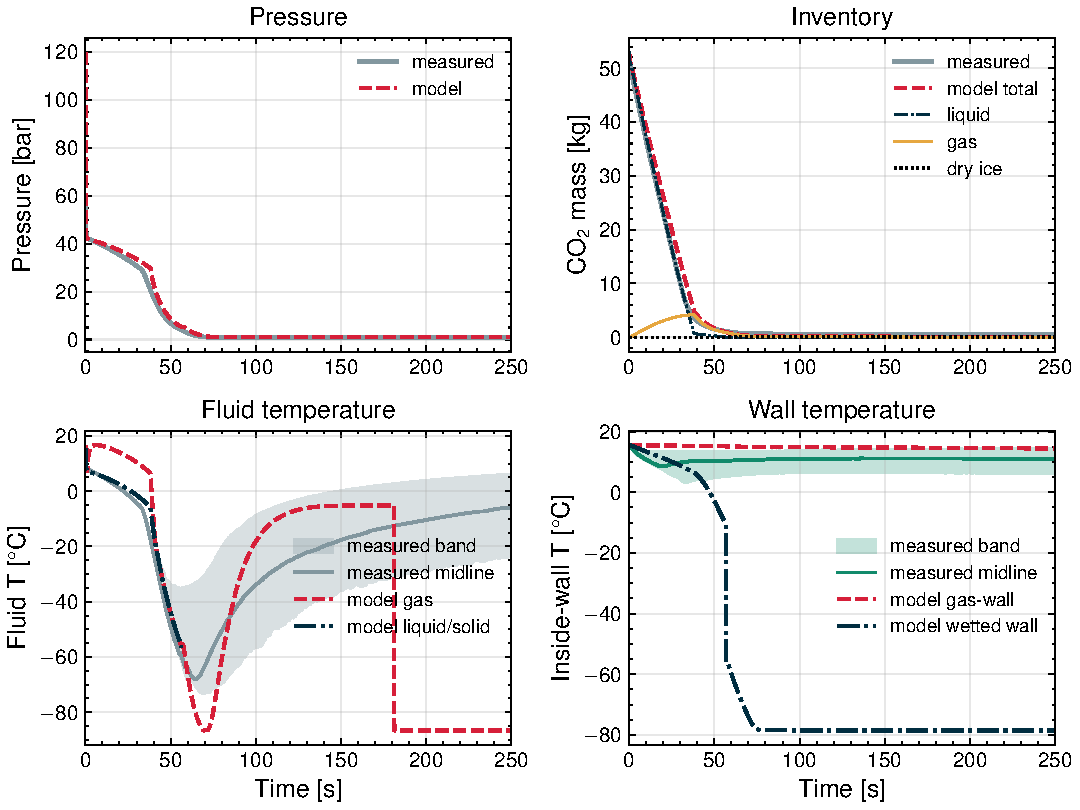
\includegraphics[width=\textwidth]{figures/munke_exp52}
\caption{SINTEF Exp52: riser (liquid), 119.9\,bar, 15.4\,$^\circ$C, 8.0\,mm nozzle.}
\label{fig:si-exp52}
\end{figure}

\begin{figure}[htbp]
\centering
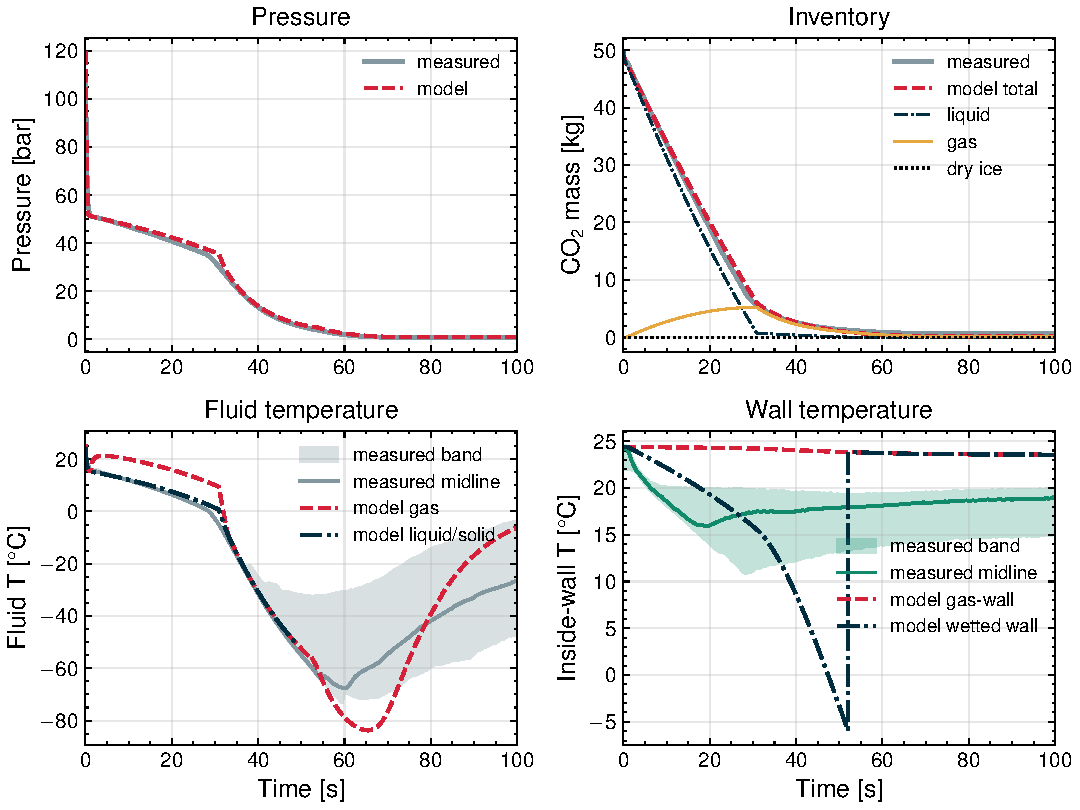
\includegraphics[width=\textwidth]{figures/munke_exp53}
\caption{SINTEF Exp53: riser (liquid), 119.5\,bar, 24.4\,$^\circ$C, 8.0\,mm nozzle (first 100\,s).}
\label{fig:si-exp53}
\end{figure}

\begin{figure}[htbp]
\centering
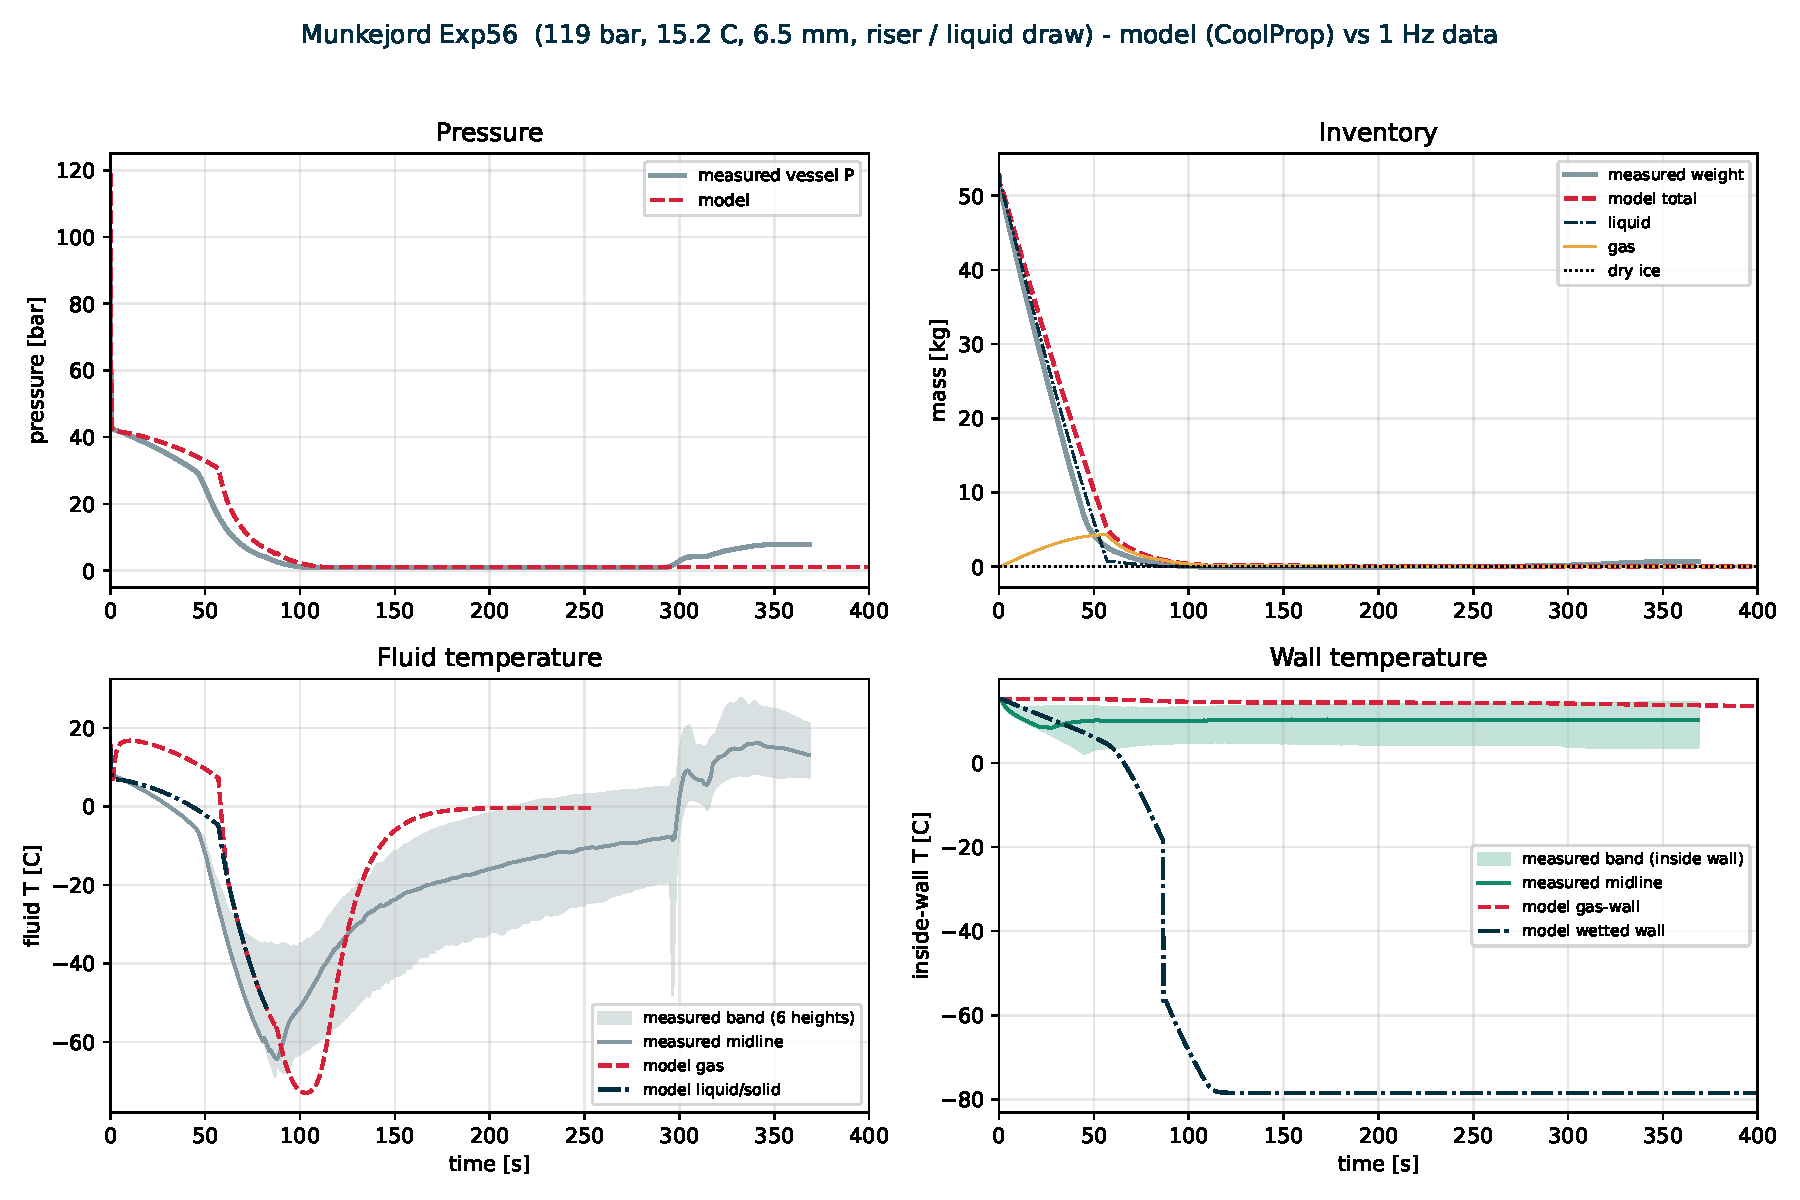
\includegraphics[width=\textwidth]{figures/munke_exp56}
\caption{SINTEF Exp56: riser (liquid), 119.1\,bar, 15.2\,$^\circ$C, 6.5\,mm nozzle.}
\label{fig:si-exp56}
\end{figure}

\begin{figure}[htbp]
\centering
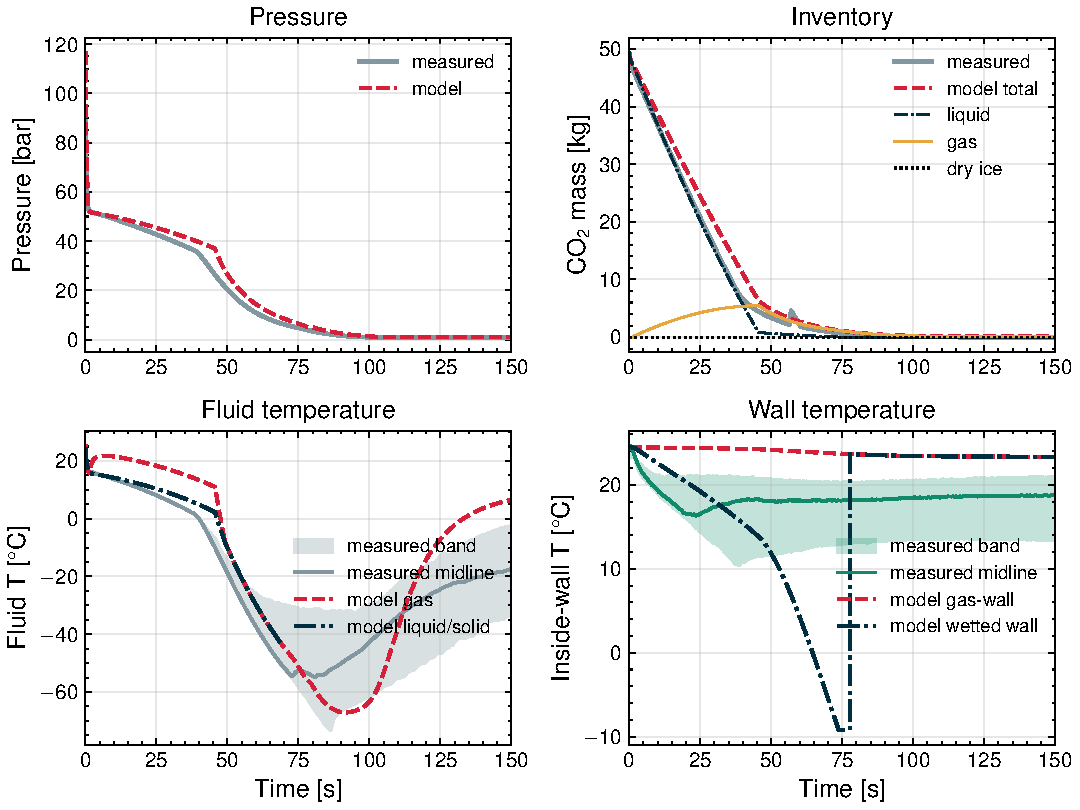
\includegraphics[width=\textwidth]{figures/munke_exp57}
\caption{SINTEF Exp57: riser (liquid), 116.8\,bar, 24.5\,$^\circ$C, 6.5\,mm nozzle (first 150\,s).
The vessel pressure is taken from the top transducer, the bottom transducer being inactive for
this test.}
\label{fig:si-exp57}
\end{figure}

\begin{figure}[htbp]
\centering
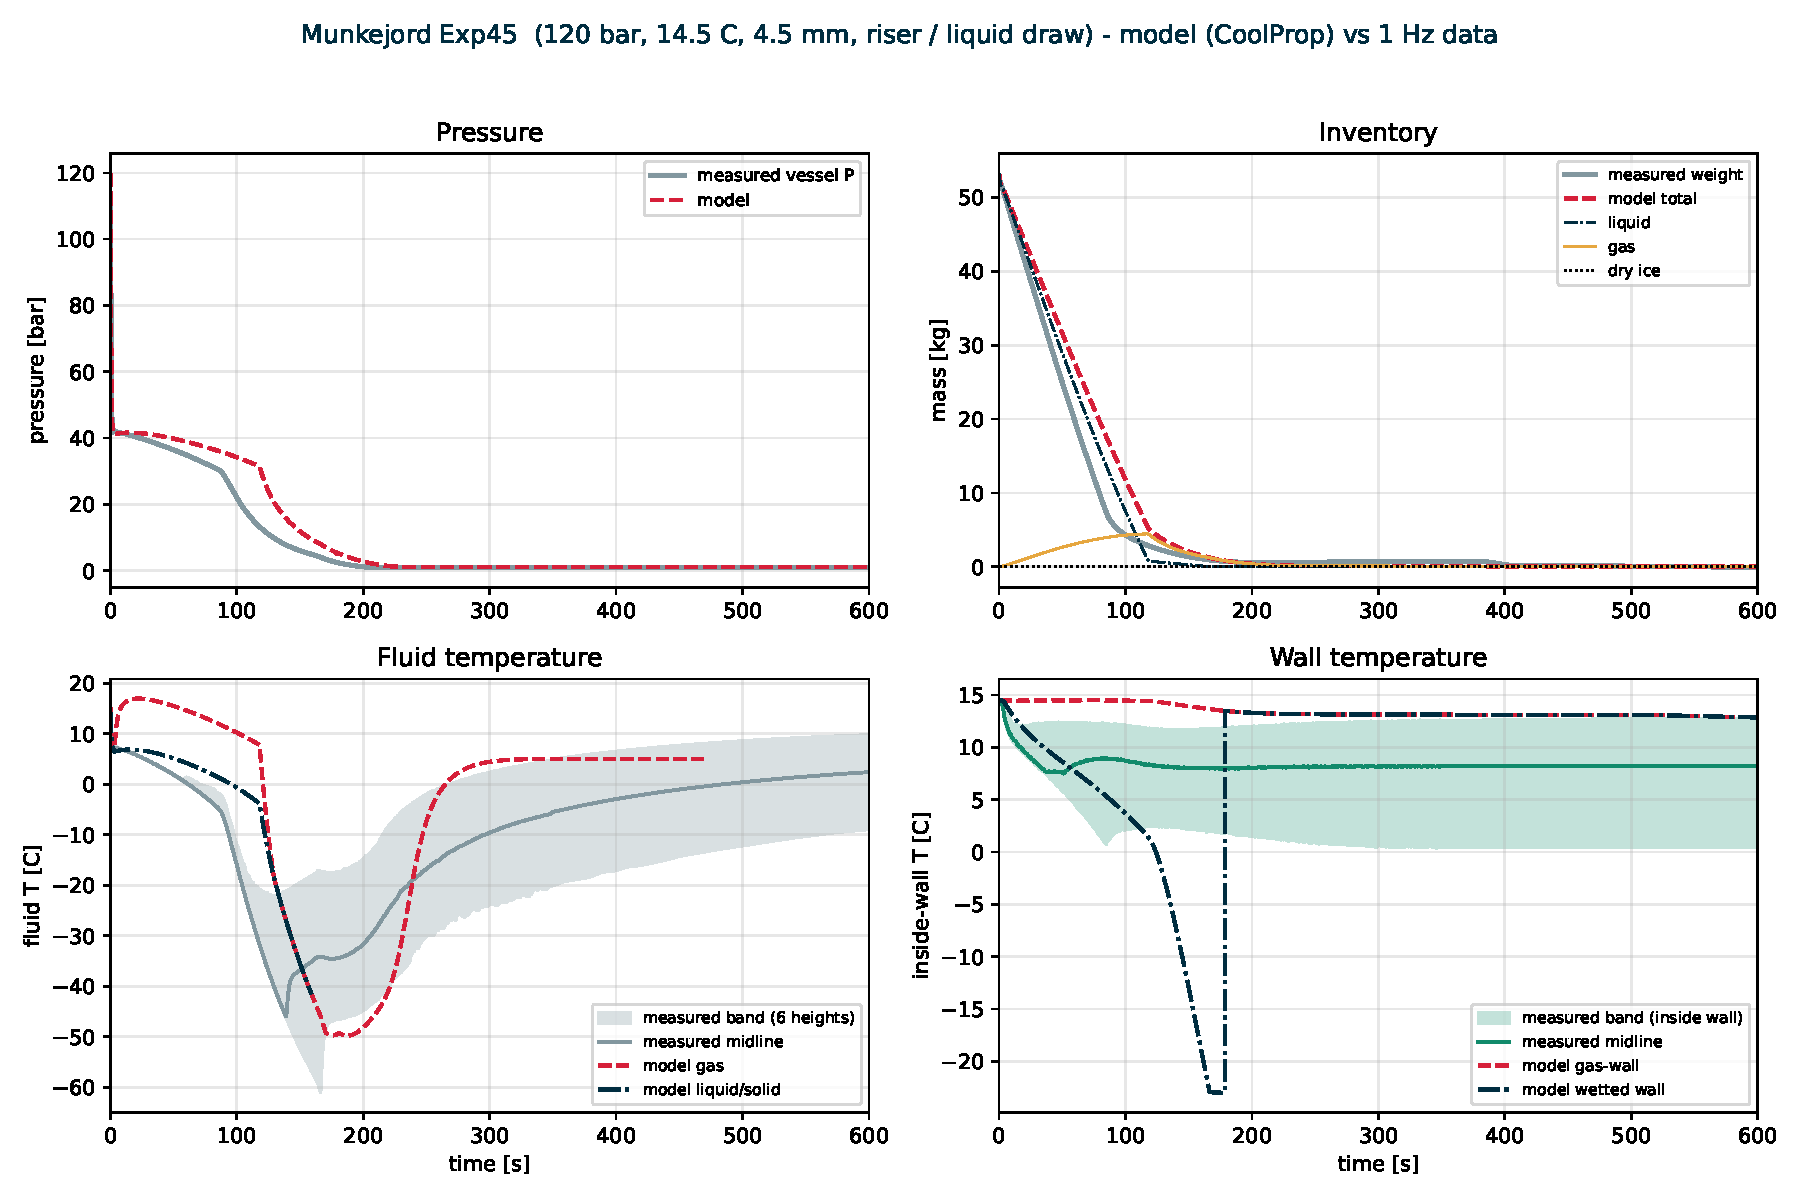
\includegraphics[width=\textwidth]{figures/munke_exp45}
\caption{SINTEF Exp45: riser (liquid), 119.9\,bar, 14.5\,$^\circ$C, 4.5\,mm nozzle.}
\label{fig:si-exp45}
\end{figure}

\begin{figure}[htbp]
\centering
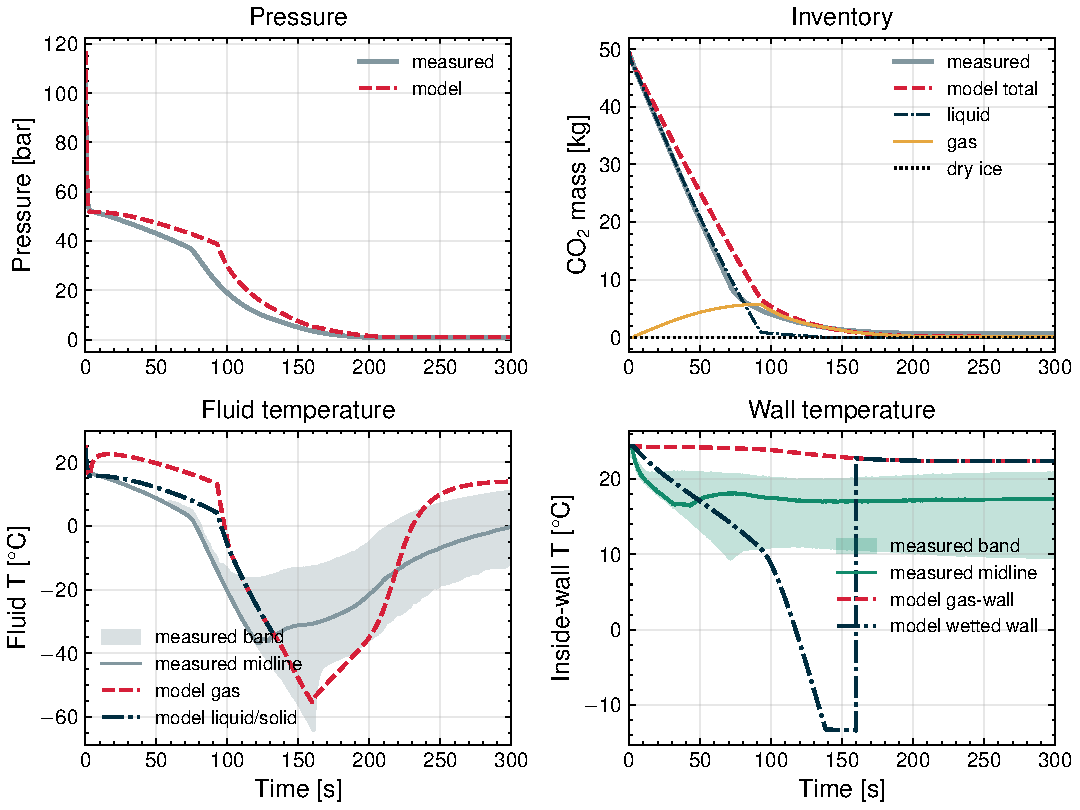
\includegraphics[width=\textwidth]{figures/munke_exp46}
\caption{SINTEF Exp46: riser (liquid), 116.7\,bar, 24.4\,$^\circ$C, 4.5\,mm nozzle (first 300\,s).}
\label{fig:si-exp46}
\end{figure}

\end{document}
